% Appendices A and B of the RQ2 paper; appendices C and D are in sections/12-appendix-cd.tex.
% Brief: outline-final.md 6.10 and Sect. 4 (Tables 3-5, Figs. 3-4). Source shorthand in the "% src:" comments:
%   DEMO  = paper/inputs/demo-materials-testing-lab-2026-11-14.json: the synthetic demo run behind Fig. 3 (offline
%           rules provider "mock", base dcat-ap-3.0.1, commit 0d7aadc; same outcome at 5ffd56e, issues digest P8)
%   DEMO5 = paper/inputs/demo-materials-testing-lab-5ffd56e-2026-11-14.json: the same demo re-run at 5ffd56e for Fig. 3;
%           metrics, dispositions and changes equal DEMO's; it adds the intake lint, the per-change checks and C8
%   ATOMS = examples/materials-testing-lab/atoms.yaml (synthetic atoms; identical at 5ffd56e)
%   @5ffd56e B/<path> = backend/profile_extensioner/<path> at commit 5ffd56e, the tool the paper describes
%   CONF5 = docs/conformance.md at 5ffd56e; RQ1 Lx = line x of the RQ1 draft text of 13 Nov 2026 (rq1-main.txt)
% No benchmark content: the atoms of Table 3 are invented, and Table 5 prints only the companion's atom counts.
% Table columns are ragged right (>{\raggedright\arraybackslash}p{}), so narrow cells do not stretch.

\section{Illustrations}\label{app:illustrations}

Table~\ref{tab:criteria} illustrates the criteria of Sect.~\ref{sec:problem}, Table~\ref{tab:checks} lists the
checks of Sect.~\ref{sec:pipeline}, and Fig.~\ref{fig:workbench} shows the workbench of Sect.~\ref{sec:impl}.

\begin{table}[tp]
  \caption{Illustrative atoms and how the criteria apply. The atoms are invented for a fictional
    materials-testing laboratory and are not benchmark content; the outcomes are those of the offline rules
    provider on \acs{DCAT-AP}~3.0.1 in the run behind Fig.~\ref{fig:workbench}, a lexical baseline, not a % src: DEMO:2-6
    model. E2: the obligation the atom's modality licenses and the one the change sets. In the run, 4 of the 15 % src: DEMO:8,10
    atoms are covered by the base and 1 is out of scope; 5 of the 10 changes are auto-accepted, and the other 5, % src: DEMO:13,20,22,72-173
    all mints at confidence 0.45, wait for review and are not compiled, so the compiled extension adds one % src: DEMO:123-172; @5ffd56e B/llm/mock.py:199; @5ffd56e B/compile/model.py:47-49
    element, tightens four and is conformant.} % src: DEMO:32-33
  \label{tab:criteria}
  \centering\scriptsize
  \setlength{\tabcolsep}{3pt}
  \begin{tabular}{@{}>{\raggedright\arraybackslash}p{3.05cm}>{\raggedright\arraybackslash}p{2.65cm}%
      >{\raggedright\arraybackslash}p{1.95cm}>{\raggedright\arraybackslash}p{1.8cm}%
      >{\raggedright\arraybackslash}p{1.9cm}@{}}
    \toprule
    Atom (modality) & E1: disposition, kind & E2: licensed / set & E3: decision & E4: against the base\\
    \midrule
    lab-01 ``Every dataset must have a title.'' (must) % src: ATOMS:19-22
      & covered by the base (B1 passed) % src: DEMO:175; a failed B1 sets the atom unclear: @5ffd56e B/engine/pipeline.py:207-211
      & mandatory / -- % src: @5ffd56e B/contracts.py:713-715
      & no change; a person may override % src: @5ffd56e B/engine/pipeline.py:538
      & inherited, no element\\
    lab-02 ``Every dataset must name the organisation responsible for making it available.'' (must) % src: ATOMS:25-28
      & refine \term{dcterms:publisher} on \term{dcat:Dataset} % src: DEMO:74,81
      & mandatory / mandatory % src: DEMO:81
      & auto-accepted; one warning to look at % src: DEMO:75,80
      & recommended $\rightarrow$ mandatory, minimum 1: tightened\\ % src: DEMO:81
    lab-06 ``A dataset should state the testing standard that the measurements followed.'' (should) % src: ATOMS:49-52
      & refine \term{dcterms:conformsTo} on \term{dcat:Dataset} % src: DEMO:104,111
      & recommended / recommended % src: DEMO:111
      & auto-accepted % src: DEMO:105,110
      & optional $\rightarrow$ recommended: tightened\\ % src: DEMO:111
    lab-07 ``A dataset should list the people who contributed to carrying out the tests.'' (should) % src: ATOMS:55-58
      & reuse \term{dcterms:contributor} on \term{dcat:Dataset} % src: DEMO:114,121
      & recommended / recommended % src: DEMO:121
      & auto-accepted % src: DEMO:115,120
      & added: the base does not constrain it there\\ % src: DEMO:33 (1 added); @5ffd56e B/engine/verify.py:319-320
    lab-11 ``A dataset must state the number of specimens that were tested.'' (must) % src: ATOMS:79-82
      & mint \term{lab:numberSpecimens}, range \term{xsd:string}: the rules provider's choice % src: DEMO:154,161; knowledge-compile-ui digest Sect. 8 item 15
      & mandatory / mandatory % src: DEMO:161
      & waits for review: confidence 0.45 below 0.5 % src: DEMO:155,160
      & added in the extension's namespace once accepted\\
    lab-12 ``A dataset must state its measurement uncertainty and the calibration date of the testing machine.''
      (must; compound) % src: ATOMS:85-88; DEMO5:623-626 (lint: compound); @5ffd56e B/engine/intake.py:72-79
      & one mint, \term{lab:measurement\allowbreak Uncertainty}; the calibration date gets no change % src: DEMO:163-172 (the only change for lab-12)
      & mandatory / mandatory % src: DEMO:171
      & waits for review (0.45) % src: DEMO:165,170
      & added in the extension's namespace once accepted\\
    lab-15 ``The portal must answer a search query within two seconds.'' (must) % src: ATOMS:103-106
      & out of scope % src: DEMO:189
      & mandatory / -- % src: @5ffd56e B/contracts.py:713-715
      & no change; a person may override % src: @5ffd56e B/engine/pipeline.py:538
      & --\\
    lab-02-cf, lab-02 with \emph{should} (counterfactual, inactive in the run) % src: ATOMS:111-118
      & expected: covered by the base % src: ATOMS:117
      & recommended / -- % src: ATOMS:114; @5ffd56e B/contracts.py:713-715
      & expected, not run % src: ATOMS:118
      & no change: the base's recommended level suffices\\ % src: ATOMS:117; DEMO:81 (base: recommended)
    \bottomrule
  \end{tabular}
\end{table}

\begin{table}[tp]
  \caption{Checks on every change (upper block) and on the compiled extension (lower block), all by program
    code except T2, a judgment of the model made only on a change without an error. Error: blocks automatic % src: @5ffd56e B/engine/pipeline.py:221-244,279
    acceptance and sends the change to repair and, if it still fails, to the queue (B1: the atom is left % src: @5ffd56e B/engine/pipeline.py:246-267,295-339
    unclear); on the extension, makes the verdict non-conformant, which blocks the sign-off. Warning: never % src: @5ffd56e B/engine/pipeline.py:207-211,618-640; @5ffd56e B/conformance/check.py:264-266
    blocking, except that a D1 warning withholds automatic acceptance by default. Source: the guideline or % src: @5ffd56e B/engine/pipeline.py:260-263; @5ffd56e B/contracts.py:606
    work followed; derived: our rule. E: the criterion served (Sect.~\ref{sec:problem}).}
  \label{tab:checks}
  \centering\scriptsize
  \setlength{\tabcolsep}{2pt}
  \begin{tabular}{@{}>{\raggedright\arraybackslash}p{1.55cm}>{\raggedright\arraybackslash}p{5.1cm}%
      >{\raggedright\arraybackslash}p{3.45cm}>{\raggedright\arraybackslash}p{0.95cm}%
      >{\raggedright\arraybackslash}p{0.55cm}@{}}
    \toprule
    Check & Error & Warning & Source & E\\
    \midrule
    V1 terms exist % src: @5ffd56e B/engine/verify.py:96-158
      & an unknown term, range or super-term; a mint outside the namespace or of an existing term; a class used
        as a property
      & a term outside the retrieved candidates; a vocabulary value that is not an IRI
      & derived & E4\\
    V2 domain and range % src: @5ffd56e B/engine/verify.py:166-211
      & a declared domain or range that excludes the class (hierarchy known); a class range on a literal
        property or the reverse
      & the same misfit, hierarchy unknown
      & derived & E4\\
    D1 DCAT version % src: @5ffd56e B/engine/verify.py:229-245,259-273; @5ffd56e B/contracts.py:606
      & a term only earlier DCAT versions define; a DCAT property without a declared domain on a class the
        base's DCAT does not list it for
      & a term only a later DCAT defines: a person decides (\emph{forbid}: error)
      & \cite[\S4]{w3cdcat3} & E4\\ % src: DCAT 3 Sect. 4, the profile definition (@5ffd56e B/data/dcat/dcat-3/spec.html:2631)
    D2 deprecation % src: @5ffd56e B/engine/verify.py:246-257
      & a term the base's DCAT or the base deprecates
      & --
      & \cite[\S4]{w3cdcat3} & E4\\ % src: DCAT 3 Sect. 4, the profile definition (@5ffd56e B/data/dcat/dcat-3/spec.html:2631)
    D3 inverses % src: @5ffd56e B/engine/verify.py:274-280; @5ffd56e B/knowledge/dcat_state.py:81,198-200; @5ffd56e B/data/dcat/dcat-3/model.json (11 pairs, 6 with a dcat: inverse; none in dcat-2014 or dcat-2)
      & --
      & every use of one of the six \term{dcat:} inverse properties (bases on DCAT~3)
      & \cite[\S7]{w3cdcat3} & E4\\ % src: DCAT 3 Sect. 7, inverse properties (@5ffd56e B/data/dcat/dcat-3/spec.html:5962-5968)
    V3 refinement % src: @5ffd56e B/engine/verify.py:291-357
      & a facet or obligation that loosens or contradicts the base; a refinement that tightens nothing
      & a facet not shown to narrow the base's
      & \cite{semicreuse2026} & E1, E4\\
    V4 reuse before mint % src: @5ffd56e B/engine/verify.py:57,365-399
      & a mint without a reason no candidate fits, a label or a definition; an indexed term of the same name
      & a candidate scoring 6.0 or more left unaddressed
      & \cite{semicreuse2026}, \cite{fathallah2026rigor,lippolis2025ontology} & E1\\
    V5 consistency % src: @5ffd56e B/engine/verify.py:407-434,493-510
      & a negative or inverted cardinality or a maximum below 1; an obligation the minimum contradicts; two
        ranges; an unfit node kind; two live changes on one class and property
      & a minted property without a range
      & derived & E1, E4\\
    T1 trace % src: @5ffd56e B/engine/verify.py:442-475
      & no atom or an inactive one; a link or facet without a reason; a quote not verbatim; an unlicensed
        obligation
      & --
      & \cite{fathallah2026rigor} & E2\\
    T2 judge % src: @5ffd56e B/engine/pipeline.py:221-244
      & unsupported, or a facet named unsupported
      & partially supported; judge unavailable
      & \cite{rashkin2023ais} & E2\\
    B1 covered by the base % src: @5ffd56e B/engine/verify.py:513-533
      & no base element named, or one not in the base or weaker than the licensed obligation
      & --
      & \cite{lippolis2025ontology} & E1\\
    \midrule
    C1 refinement % src: @5ffd56e B/conformance/check.py:111-142 (obligation compared only where the base has a shape: :119-120)
      & a loosened constraint or obligation (obligations only where the base has a shape)
      & --
      & \cite{semicreuse2026} & E4\\
    C2 no contradiction % src: @5ffd56e B/conformance/check.py:143-147; @5ffd56e B/conformance/refinement.py:116,128,133,166,177,195; CONF5:44
      & unsatisfiable with the base: crossing bounds, another datatype, disjoint node kinds or value lists
      & --
      & derived & E4\\
    C3 own namespace % src: @5ffd56e B/conformance/check.py:149-158
      & a mint outside the extension's namespace or of an existing term
      & --
      & \cite{semicreuse2026} & E4\\
    C4 existing terms % src: @5ffd56e B/conformance/check.py:160-168
      & a reused property that is not in the vocabulary index
      & --
      & derived & E4\\
    C5 trace % src: @5ffd56e B/conformance/check.py:170-177
      & an element without an atom, or with an inactive one
      & --
      & \cite{semicreuse2026} & E2\\
    C6 (V6) SHACL % src: @5ffd56e B/engine/verify.py:536-549; @5ffd56e B/conformance/check.py:254-255
      & shapes that do not parse or fail the SHACL shapes for SHACL
      & --
      & \cite{w3cshacl} & E4\\
    C7 witness % src: @5ffd56e B/conformance/check.py:212-247,257-261; base-only branch unreachable: knowledge-compile-ui digest Sect. 4.4
      & -- (its base-only branch cannot fire)
      & the witness fails base and extension (Sect.~\ref{sec:compile}) or does not run
      & derived & E4\\
    C8 DCAT state % src: @5ffd56e B/conformance/check.py:64-99
      & a DCAT term the base's DCAT deprecates or no longer defines
      & a later DCAT term, by default accepted only by a person
      & \cite[\S4]{w3cdcat3} & E4\\ % src: DCAT 3 Sect. 4, the profile definition (@5ffd56e B/data/dcat/dcat-3/spec.html:2631)
    \bottomrule
  \end{tabular}
\end{table}

% Workbench figure (appendix). Screenshots of the synthetic demo examples/materials-testing-lab/atoms.yaml
% with the offline rules provider (mock), retaken on 14 Nov 2026 at commit 5ffd56e (the tool the paper describes;
% frontend built from that commit); numbers in paper/inputs/demo-materials-testing-lab-5ffd56e-2026-11-14.json, equal to
% those of the first take at 0d7aadc (paper/inputs/demo-materials-testing-lab-2026-11-14.json). No benchmark content.
\begin{figure}[!htbp]
  \centering
  \begin{minipage}[t]{0.485\textwidth}
    \vspace{0pt}
    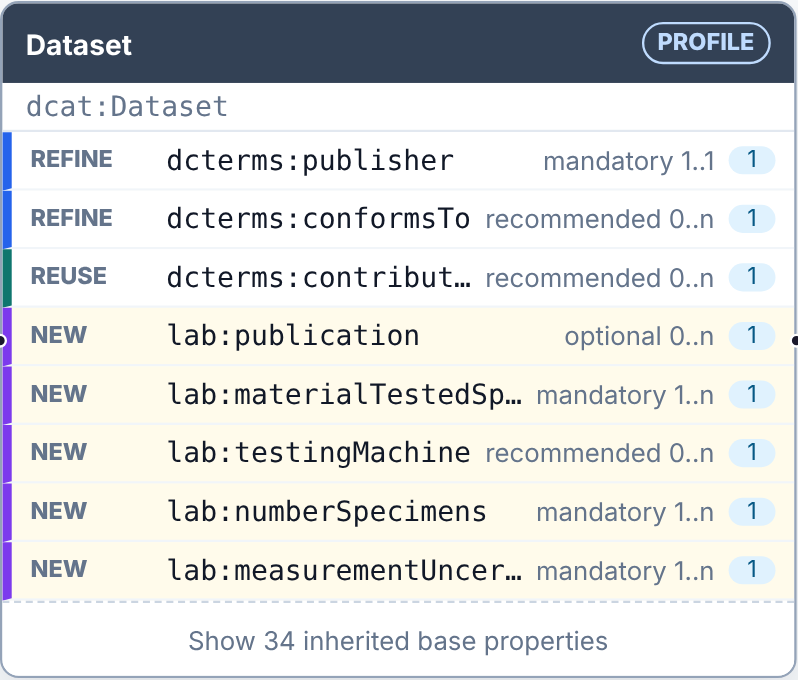
\includegraphics[width=\linewidth]{figures/wb-canvas-dataset.png}\\[0.6ex]
    {\scriptsize (a) Canvas card of \term{dcat:Dataset}}\\[1.2ex]
    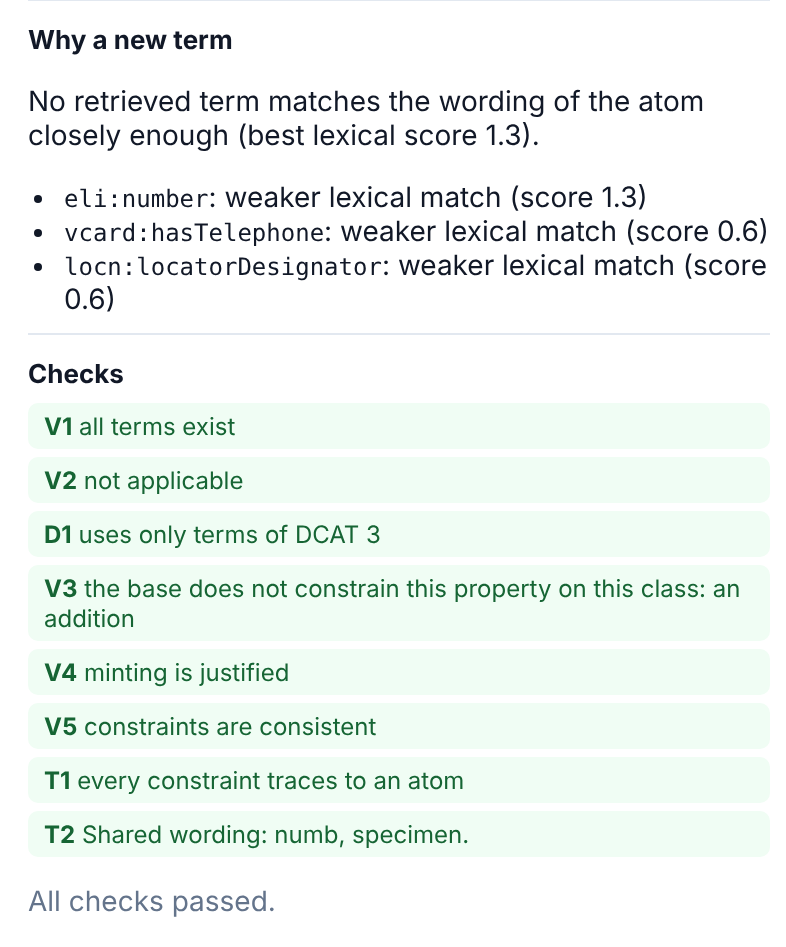
\includegraphics[width=\linewidth]{figures/wb-inspector-mint-bottom.png}\\[0.6ex]
    {\scriptsize (c) Inspector, continued: rejected candidates and checks}
  \end{minipage}\hfill
  \begin{minipage}[t]{0.485\textwidth}
    \vspace{0pt}
    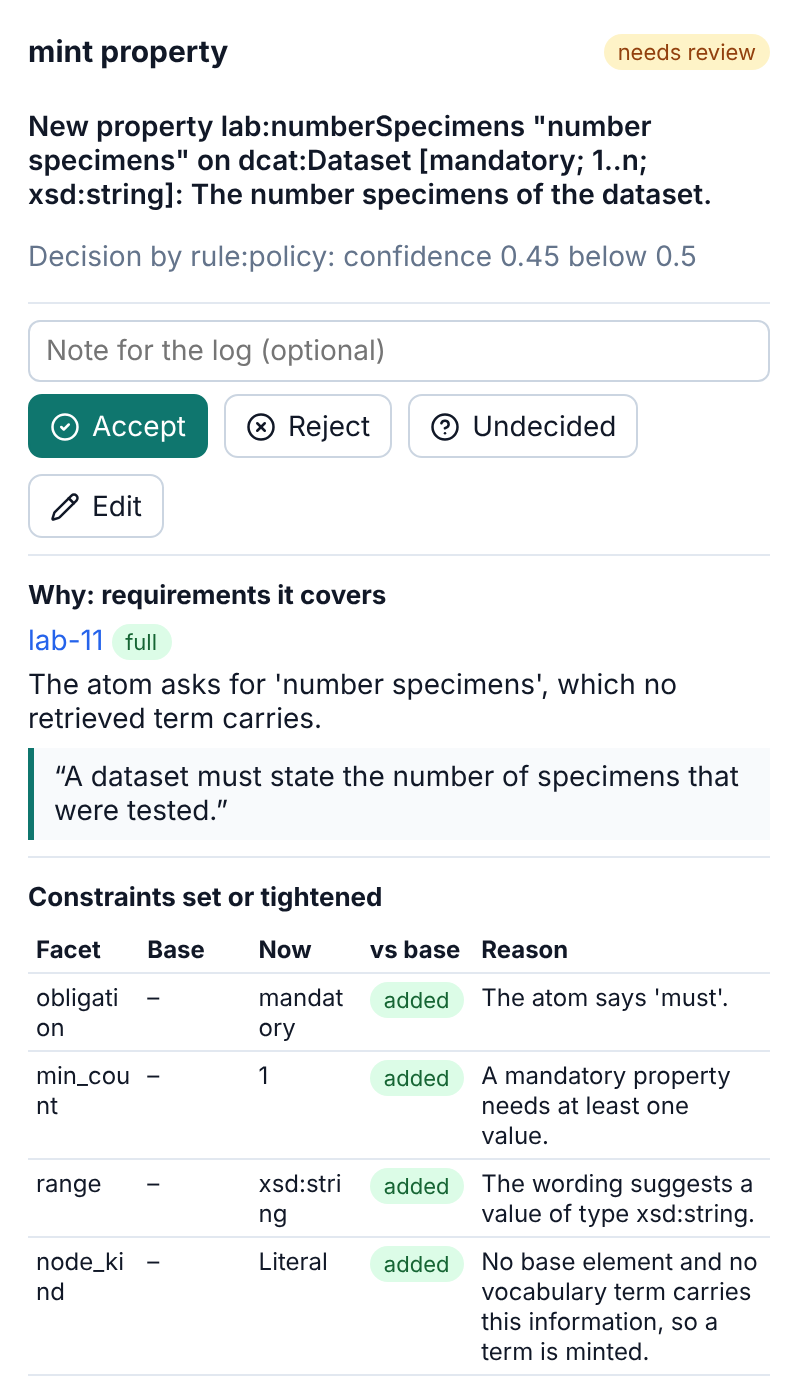
\includegraphics[width=\linewidth]{figures/wb-inspector-mint-top.png}\\[0.6ex]
    {\scriptsize (b) Inspector of one minted property}
  \end{minipage}
  \caption{The workbench on the synthetic demo of Table~\ref{tab:criteria}, run with the offline rules provider
    instead of a model, so the choices shown are a lexical baseline's (\term{xsd:string} for a count).
    (a)~Rows that tighten a base constraint (REFINE), add an existing term (REUSE) or mint one (NEW),
    with obligation, cardinality and atoms covered; shaded rows wait for review. (b)~The decision and why the
    machine left it open, the covered atom with its verbatim quote, and one justification per constraint, with
    base and new value. (c)~The candidates the mint rejected, with their lexical scores, and the checks.}
  \label{fig:workbench}
\end{figure}


\section{The Benchmark in Full}\label{app:benchmark}

Table~\ref{tab:cases-full} lists the cases in full, and Fig.~\ref{fig:reference} shows how a reference delta is built
and matched (Sect.~\ref{sec:benchmark}). \todo{cases in full: base release and reference version per case (Q3);
source of each reference delta (Q23); elements by kind; aligned elements (Q9); A-rq1 (Q21); counterfactual atoms
per case; test-case atom counts as in Table~\ref{tab:cases} (Q11)}

\begin{table}[tp]
  \caption{The five cases in full, test cases above development cases. Base: the release the reference delta is
    computed against. Reference: the published profile and its version; in parentheses, how the reference delta
    is obtained, shapes compared or tables extracted by hand. Elements: reference elements by kind; loosened:
    elements that relax the base, reported apart. Aligned: elements at least one atom asks for (in parentheses,
    those none asks for). Atoms: A-gold, the scored content atoms of the companion benchmark
    \cite{anon2027rq1}; A-rq1, atoms converted from the needs of the companion workflow; counterfactual, atoms
    reworded so that the right answer departs from the publication.}
  \label{tab:cases-full}
  \centering\scriptsize
  \setlength{\tabcolsep}{2.5pt}
  \begin{tabular}{@{}>{\raggedright\arraybackslash}p{1.95cm}>{\raggedright\arraybackslash}p{1.3cm}rrrrrrrrr@{}}
    \toprule
    & & \multicolumn{4}{c}{Elements} & & & \multicolumn{3}{c}{Atoms}\\
    \cmidrule(lr){3-6}\cmidrule(l){9-11}
    Case (base) & Reference (source) & reuse & refine & mint & class & loosened & Aligned & A-gold & A-rq1
      & counterf.\\
    \midrule
    % Base, reference and source: author decisions (Q3, Q23), \tbd here. Counts: \res slots for the RQ2 evaluator
    % (scopes as in Table 2: mobility, geo, health, test, stat, jrc, five; condition "all"); they print \tbd until
    % defined. A-gold: the companion's scored content atoms (RQ1 Table 1, "Atoms").
    mobilityDCAT-AP (\tbd) & \tbd{} (\tbd) & \res{mobility}{all}{reuse} & \res{mobility}{all}{refine} & \res{mobility}{all}{mint} & \res{mobility}{all}{class} & \res{mobility}{all}{loosened}
      & \res{mobility}{all}{N} (\res{mobility}{all}{unaligned}) & 39 % src: RQ1 L382 (Table 1, Atoms)
      & \res{mobility}{all}{arq1} & \res{mobility}{all}{counterfactual}\\
    GeoDCAT-AP (\tbd) & \tbd{} (\tbd) & \res{geo}{all}{reuse} & \res{geo}{all}{refine} & \res{geo}{all}{mint} & \res{geo}{all}{class} & \res{geo}{all}{loosened}
      & \res{geo}{all}{N} (\res{geo}{all}{unaligned}) & 37 % src: RQ1 L383
      & \res{geo}{all}{arq1} & \res{geo}{all}{counterfactual}\\
    HealthDCAT-AP (\tbd) & \tbd{} (\tbd) & \res{health}{all}{reuse} & \res{health}{all}{refine} & \res{health}{all}{mint} & \res{health}{all}{class} & \res{health}{all}{loosened}
      & \res{health}{all}{N} (\res{health}{all}{unaligned}) & 89 % src: RQ1 L384
      & \res{health}{all}{arq1} & \res{health}{all}{counterfactual}\\
    \textit{Test cases} &  & \res{test}{all}{reuse} & \res{test}{all}{refine} & \res{test}{all}{mint} & \res{test}{all}{class} & \res{test}{all}{loosened}
      & \res{test}{all}{N} (\res{test}{all}{unaligned}) & 165 % src: RQ1 L385 (39+37+89)
      & \res{test}{all}{arq1} & \res{test}{all}{counterfactual}\\
    \midrule
    StatDCAT-AP (\tbd) & \tbd{} (\tbd) & \res{stat}{all}{reuse} & \res{stat}{all}{refine} & \res{stat}{all}{mint} & \res{stat}{all}{class} & \res{stat}{all}{loosened}
      & \res{stat}{all}{N} (\res{stat}{all}{unaligned}) & 14 % src: RQ1 L386
      & \res{stat}{all}{arq1} & \res{stat}{all}{counterfactual}\\
    DCAT-AP-JRC (\tbd) & \tbd{} (\tbd) & \res{jrc}{all}{reuse} & \res{jrc}{all}{refine} & \res{jrc}{all}{mint} & \res{jrc}{all}{class} & \res{jrc}{all}{loosened}
      & \res{jrc}{all}{N} (\res{jrc}{all}{unaligned}) & 17 % src: RQ1 L387
      & \res{jrc}{all}{arq1} & \res{jrc}{all}{counterfactual}\\
    \midrule
    All five &  & \res{five}{all}{reuse} & \res{five}{all}{refine} & \res{five}{all}{mint} & \res{five}{all}{class} & \res{five}{all}{loosened}
      & \res{five}{all}{N} (\res{five}{all}{unaligned}) & 196 % src: RQ1 L388 (165+14+17)
      & \res{five}{all}{arq1} & \res{five}{all}{counterfactual}\\
    \bottomrule
  \end{tabular}
\end{table}

\begin{figure}[tp]
  \centering
  % Fig. 4: from a published profile to Recovery (appendix B). Mirrors the RQ1 paper's Fig. 4: seven numbered steps
% in a zigzag (1-3 left to right, 4-6 right to left, 7 below), the final box filled, and a dashed path from the steps
% that set elements apart into a dashed box for what stays outside the denominator. Node and arrow styles follow
% figures/pipeline.tex. Box texts: outline-final.md, brief 6.10 (Fig. 4). Input inside a figure environment
% (sections/11-appendix.tex), which holds the caption and the label fig:reference.
\begin{tikzpicture}[
    font=\scriptsize,
    op/.style={draw, rounded corners=2pt, minimum height=1.05cm, align=center,
               inner sep=2pt, text width=3.4cm},
    final/.style={op, fill=black!8, text width=7.4cm},
    outside/.style={op, dashed},
    flow/.style={-{Stealth[length=1.5mm]}, semithick},
    side/.style={-{Stealth[length=1.5mm]}, semithick, dashed},
  ]
  % row 1: build the reference delta (left to right)
  \node[op] (s1) at (0,0)   {1.\ Pin the base release, its DCAT version and the published profile};
  \node[op] (s2) at (4,0)   {2.\ Compare shapes and obligation tables per (class, property), or extract tables by hand};
  \node[op] (s3) at (8,0)   {3.\ Drop inherited constraints, classify by kind, set loosened elements apart};
  % row 2: fix the denominator, then match (right to left)
  \node[op] (s4) at (8,-1.65) {4.\ Align atoms to the\\ elements they ask for};
  \node[op] (s5) at (4,-1.65) {5.\ Freeze the\\ reference deltas};
  \node[op] (s6) at (0,-1.65) {6.\ Match included changes:\\ strict, relaxed, by meaning};
  % row 3: the report (filled) and what stays outside the denominator (dashed)
  \coordinate (r3) at (0,-3.4);
  \node[final, anchor=west] (s7) at (s6.west |- r3)
        {7.\ Report Recovery:\\ aligned elements with a match / aligned elements;\\ Strict beside it};
  \node[outside] (out) at (8,-3.4)
        {Outside the denominator: elements no atom asks for, loosened elements, usage notes, unhandled constructs};
  % solid path
  \draw[flow] (s1) -- (s2);
  \draw[flow] (s2) -- (s3);
  \draw[flow] (s3) -- (s4);
  \draw[flow] (s4) -- (s5);
  \draw[flow] (s5) -- (s6);
  \draw[flow] (s6.south) -- (s6.south |- s7.north);
  % dashed path: elements set apart in step 3 and left unaligned in step 4
  \coordinate (bus) at ([xshift=3mm]s3.east);
  \draw[side] (s3.east) -- (bus) |- (out.east);
  \draw[semithick, dashed] (s4.east) -- (s4.east -| bus);
\end{tikzpicture}

  \caption{From a published profile to Recovery, in the order of the arrows. Steps 1 to 5 fix the denominator,
    the aligned reference elements, before step 6 matches any output; the dashed path collects what stays
    outside it. Strict is reported beside Recovery.}
  \label{fig:reference}
\end{figure}
